\chapter{计划进度和预期成果}

本项目预计在中期前完成所有组件的开发和测试工作，并搭建双板的一个小型的多FPGA硬件仿真系统进行初步的测试和评估。中期后会进行规模扩大和性能调优，编写毕业论文等相关事宜。具体时间安排如图~\ref{fig:project_timeline}所示：

\begin{figure}[htb]
    \centering
    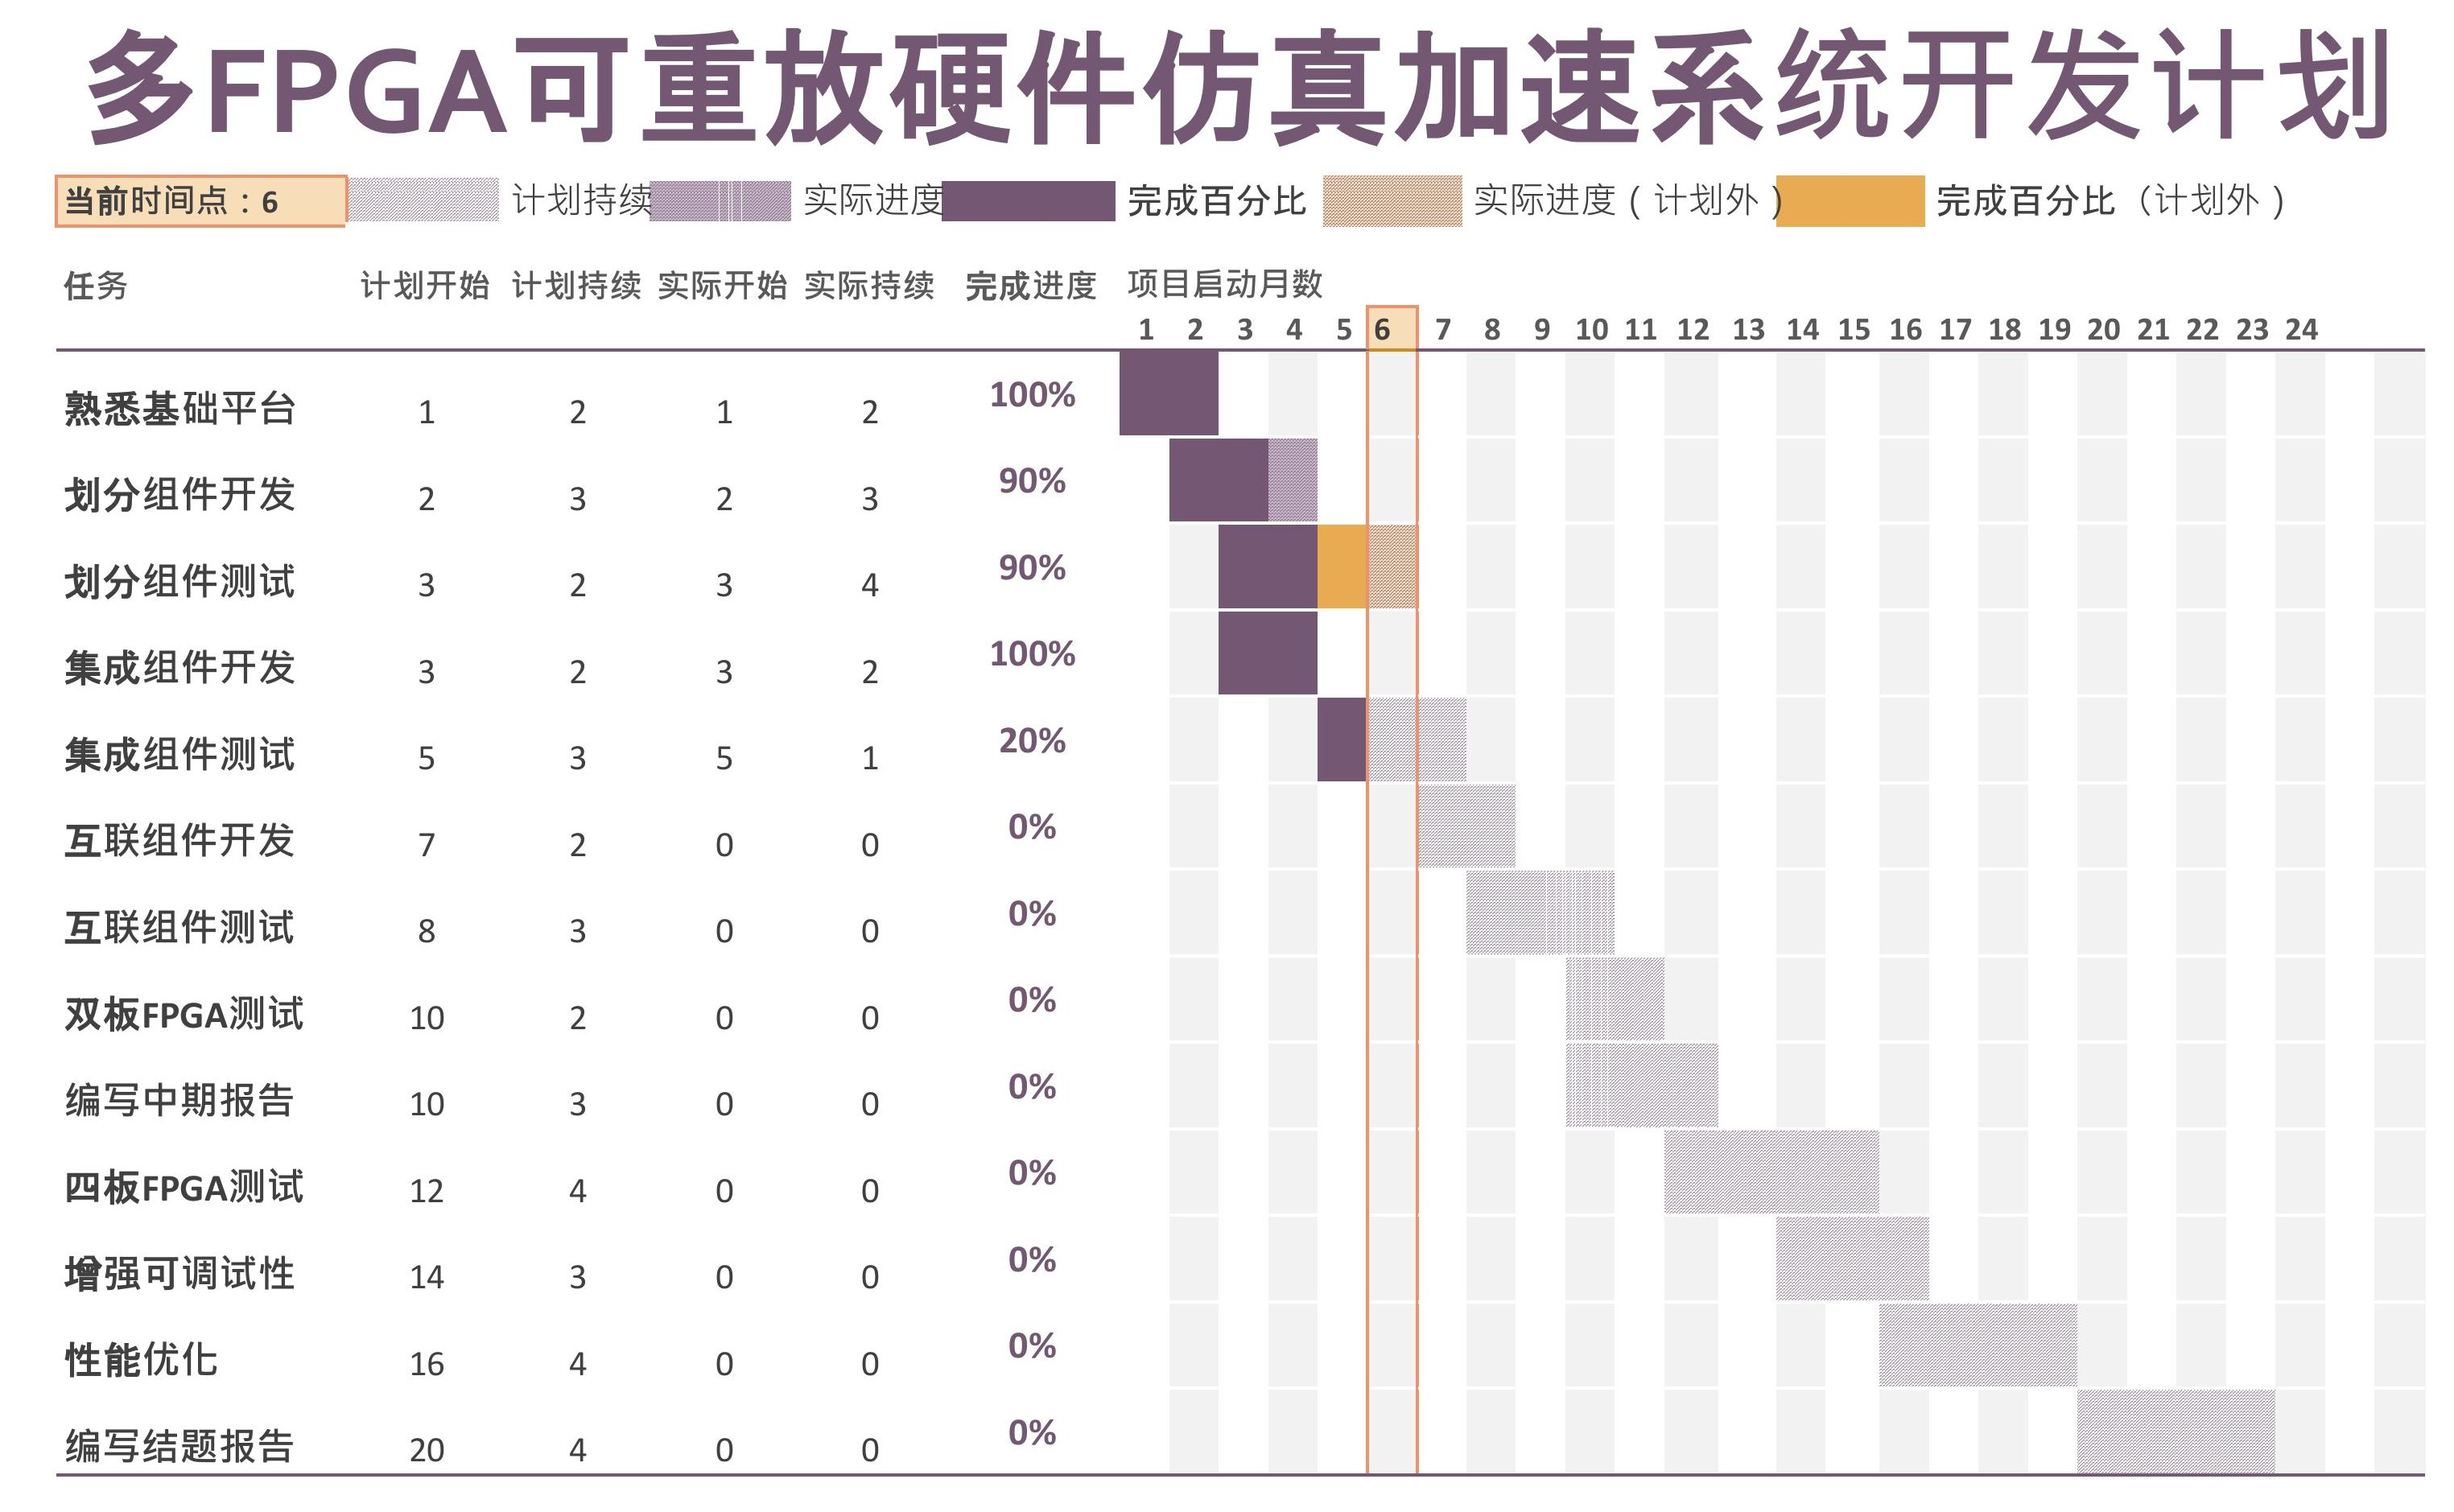
\includegraphics[width=\columnwidth]{figure/plan.jpg}
    \bicaption{项目计划时间表}{Project Timeline}
    \label{fig:project_timeline}
\end{figure}

目前已经完成了划分组件的开发和测试、跨边界接口组件的开发、互连组件的开发。预计在中期，得到一个可以稳定运行的2个FPGA硬件仿真系统，系统上部署了Picorv32为CPU的小型SoC，处理器运行裸机程序，能够实现暂停、波形重放等主要的调试功能。在结题阶段，展示一个可以5MHz运行的4个FPGA的硬件仿真系统，部署一个四核的香山昆明湖处理器和相应外设，支持波形重放、Trace等全部调试功能，能够运行并调试操作系统和应用程序。